%%%%%%%%%%%%%%%%%%%%%%%
%%% DOCUMENT SETTINGS
%%%%%%%%%%%%%%%%%%%%%%%
\documentclass[11pt]{exam}
\printanswers % Uncomment to show answers
%%%%%%%%%%%%%%
%%% PACKAGES
%%%%%%%%%%%%%%
\usepackage{amsmath,amsfonts,amssymb,amsthm} % math fonts and symbols
\usepackage{bbm} % Math blackboard font
\usepackage{enumitem} % For reference enumerations lists
\usepackage{textcomp} % some symbols (like copyright)
\usepackage[top = 2cm, bottom = 2cm, right = 1.2cm, left = 1.2cm, paper = a4paper, headheight = 6cm]{geometry} % Margins setup
\usepackage{xcolor} % Colors
\usepackage{graphicx}
%----------------------------------- Tikz
\usepackage{tikz}
\usepackage{pgfplots}
\pgfplotsset{compat=1.17}
\usepgfplotslibrary{fillbetween}
\usetikzlibrary{shapes,arrows,matrix,positioning,calc}
\newcommand{\tikzmark}[1]{\tikz[baseline,remember picture] \coordinate (#1) {};}
%%%%%%%%%%%%%%%%%%%%%%%%%%
%%% Colors
%%%%%%%%%%%%%%%%%%%%%%%%%%
\definecolor{firebrick3}{RGB}{207, 33, 32}
\definecolor{deepskyblue3}{RGB}{0, 155, 206}
\definecolor{darkolivegreen3}{RGB}{163, 207, 91}
%%%%%%%%%%%%%%%%%%%%%%%%%%
%%% MACROS AND COMMANDS
%%%%%%%%%%%%%%%%%%%%%%%%%%
\newcommand{\N}{\mathbb{N}} % natural number set
\newcommand{\R}{\mathbb{R}} % real number set
\makeatletter
\renewcommand{\@makefnmark}{\textsuperscript{\arabic{footnote}}} % Ensure numeric superscripts
\renewcommand{\thefootnote}{\arabic{footnote}} % Ensure numeric labels
\makeatother
\setcounter{footnote}{0}
\newcommand{\BAR}{%
    \hspace{-\arraycolsep}%
    \strut\vrule % the `\vrule` is as high and deep as a strut
    \hspace{-\arraycolsep}%
}
%%%%%%%%%%%%%%%%%%%%%%%%%%%%%%%%%
%%% HEADER AND FOOT 
%%%%%%%%%%%%%%%%%%%%%%%%%%%%%%%%%
% Defining information
\newcommand{\degree}{Bachelor in Philosophy, Politics and Economics}
\newcommand{\shortdeg}{PPE}
\newcommand{\exam}{Final Exam}
\newcommand{\subject}{Mathematics}
\newcommand{\theyear}{2025/26}
\newcommand{\ccauthor}{A. G. Azze}
\newcommand{\thedate}{Dec 12, 2025}
\newcommand{\university}{CUNEF Universidad}
% Setting header and footer
\pagestyle{headandfoot}
\header{\degree \\ \subject\ - \theyear}{}{\thedate \\ \ccauthor}
\footer{\university}{}{\thepage}
%%%%%%%%%%%%%%%%%%%%%%%%%
%%% DOCUMENT CONTENT
%%%%%%%%%%%%%%%%%%%%%%%%%
\begin{document}
%--- Instructions ---%
\begin{center}

    {\Huge \textbf{\exam{}}}
   

    \begin{flushright}
        \vspace{-0.3cm}
        \textbf{Time Limit:} 120 minutes
    \end{flushright}
    \vspace{-0.15cm}
    
    \fbox{\parbox{\textwidth}{\centering 
        \begin{enumerate}[leftmargin = 0.5cm, label = $\bullet$, rightmargin = 0.2cm]
    
            \item \textbf{Every non-trivial calculation and claim in the exam must be properly justified.}

            \item The use of calculators is not necessary and therefore not allowed.

            \item Digital devices such as mobile phones, tablets, and laptops, as well as internet access, are forbidden.
            
        \end{enumerate}
    }}
\end{center}
%--- Instructions ---%

%--- Questions ---%

\begin{questions}

% Question
\question[2]
The AI market is described by the supply and demand functions $p_S(q) = 5e^{q - 1}$ and $p_D(q) = \frac{10}{1 + q^2}$.

\begin{minipage}{0.6\textwidth}
    \begin{enumerate}[leftmargin = 0.5cm, label = (\alph*), rightmargin = 0.2cm]
        \item Prove that there is an equilibrium at $p^* = 5$. Find $q^*$.
        \item Provided that the Total Consumer Value (TCV) is given by
        $$
        TCV = \int_0^{q^*} \frac{10}{1 + q^2}\, \mathrm{d} q = 7.85,
        $$
        Compute the area $C$ in Figure 1.
        \item Compute the area denoted by $A$ in Figure 1, provided that 
        $$
        \int_{q^*}^{2} \frac{10}{1 + q^2}\, \mathrm{d} q = 3.22.
        $$
        \item Provide an estimate of $p_S(1.1)$ using the tangent line at $q = 1$.
    \end{enumerate}
\end{minipage}
\hspace{0.5cm}
\begin{minipage}{0.34\textwidth}
    \vspace{-0.5cm}
    
    \begin{center}
    
    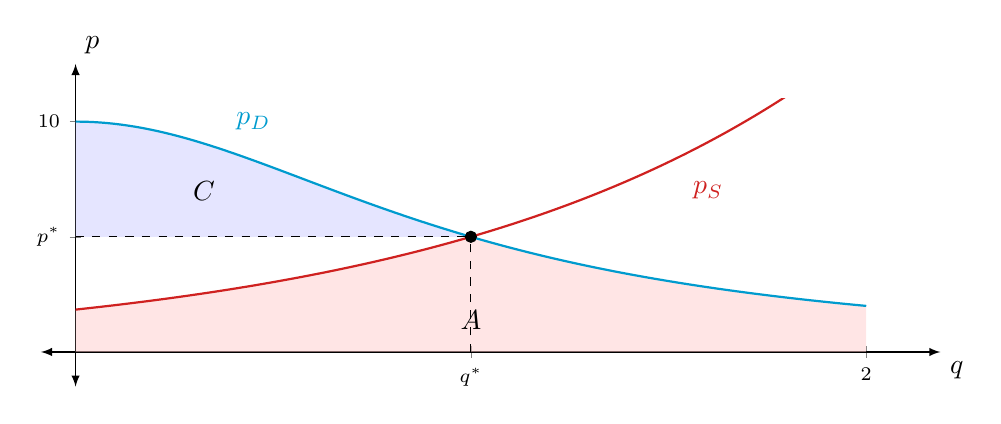
\begin{tikzpicture}
    \begin{axis}[
        width=\textwidth,
        height=4.8cm,
        axis lines=middle,
        xmin=0,
        xmax=2.1,
        ymin=0,
        ymax=11,
        ytick={0,5,10},
        xtick={0,1,2},
        xticklabels={$0$, $q^*$, $2$}, % Custom x-tick labels
        yticklabels={$0$, $p^*$, $10$}, % Custom y-tick labels
        scaled ticks = false,
        ticklabel style={font=\scriptsize},
        xlabel=$q$,
        ylabel=$p$,
        axis line style={
            latex-latex,
            shorten >=-12.5pt,
            shorten <=-12.5pt,
        },
        xlabel style={at={(ticklabel* cs:1)}, xshift=12.5pt, anchor=north west},
        ylabel style={at={(ticklabel* cs:1)}, yshift=12.5pt, anchor=south west},
    ]

    % Demand curve from 0 to q* (for consumer surplus)
    \path[name path=demand_left] 
        plot[smooth, domain=0:1] (\x, {10/(1 + \x^2)});
    % Price line at p* from 0 to q*
    \path[name path=price] (axis cs:0,5) -- (axis cs:1,5);

    % Consumer surplus area C
    \addplot[fill=blue!20, opacity=0.5] fill between[
        of=demand_left and price,
    ];

    % Supply curve from 0 to q*
    \path[name path=supply] 
        plot[smooth, domain=0:1] (\x, {5*exp(\x - 1)});
    % x-axis baseline for supply (0 to q*)
    \path[name path=xaxis_supply] (axis cs:0,0) -- (axis cs:1,0);

    % Demand curve from q* to 2
    \path[name path=demand_right] 
        plot[smooth, domain=1:2] (\x, {10/(1 + \x^2)});
    % x-axis baseline for demand from q* to 2
    \path[name path=xaxis_demand] (axis cs:1,0) -- (axis cs:2,0);

    % Area A: under supply from 0 to q* and under demand from q* to 2
    \addplot[fill=red!20, opacity=0.5] fill between[
        of=supply and xaxis_supply,
    ];
    \addplot[fill=red!20, opacity=0.5] fill between[
        of=demand_right and xaxis_demand,
    ];

    % Supply and demand functions
    \addplot[thick, firebrick3, samples=101, smooth, domain=0:2] 
        {5*exp(x - 1)};
    \addplot[thick, deepskyblue3, samples=101, smooth, domain=0:2] 
        {10/(1 + x^2)};

    % Equilibrium point (q*, p*) = (1, 5)
    \addplot[mark=*] coordinates {(1,5)} node[] {};

    % Dashed lines to the equilibrium point
    \addplot[dashed] coordinates {(1,0) (1,5)}; % Vertical line
    \addplot[dashed] coordinates {(0,5) (1,5)}; % Horizontal line

    % Function labels
    \addplot[] coordinates {(1.6,7)} node[] {$\textcolor{firebrick3}{p_S}$};
    \addplot[] coordinates {(0.45,10)} node[] {$\textcolor{deepskyblue3}{p_D}$};

    % Area labels
    \addplot[] coordinates {(0.325,7)} node[] {$C$};
    \addplot[] coordinates {(1,1.4)} node[] {$A$};

    \end{axis}
\end{tikzpicture}
    % \vspace{-0.6cm}
    
    {\small Figure 1}
    \end{center}        
\end{minipage}
    
% Solution
\begin{solution}[0cm]
\begin{enumerate}[leftmargin = 0.5cm, label = (\alph*), rightmargin = 0.2cm]

    \item 
    From demand:
    \[
        p_D(q) = 5 
        \;\Rightarrow\; \frac{10}{1+q^2} = 5 
        \;\Rightarrow\; 1 + q^2 = 2 
        \;\Rightarrow\; q^2 = 1 
        \;\Rightarrow\; q = 1 \quad (q \ge 0).
    \]
    From supply:
    \[
        p_S(q) = 5 
        \;\Rightarrow\; 5e^{q-1} = 5 
        \;\Rightarrow\; e^{q-1} = 1 
        \;\Rightarrow\; q - 1 = 0 
        \;\Rightarrow\; q = 1.
    \]
    Thus both curves give $p = 5$ at $q = 1$, so $(q^*,p^*) = (1,5)$.

    \item Given $TCV = 7.85$,
    \[
        C = \int_0^{q^*} \bigl(p_D(q) - p^*\bigr)\,dq
          = \int_0^{1} \frac{10}{1+q^2}\,dq - \int_0^{1} 5\,dq
          = TCV - 5 = 2.85
    \]

    \item 
    From the figure, $A$ is the area under the supply curve from $0$ to $1$ plus the area under the demand curve from $1$ to $2$:
    \[
        A = \int_0^{1} 5e^{q-1}\,dq \;+\; \int_1^{2} \frac{10}{1+q^2}\,dq.
    \]

    First integral:
    \[
        \int_0^{1} 5e^{q-1}\,dq 
        = 5 \int_0^{1} e^{q-1}\,dq
        = 5\bigl[e^{q-1}\bigr]_0^{1}
        = 5(1 - e^{-1}) 
        = 5 - \frac{5}{e}
        \approx 3.16.
    \]
    Hence,
    \[
        A = 5 - \frac{5}{e} + 3.22 = 8.22 - \frac{5}{e}.
    \]

    \item Since $p_S'(q) = 5e^{q-1}$, we have that
    $$
    p_S(1.1) \approx p_S(1) + p_S'(1)\times0.1 = 5 + 5\times 0.1 = 5.5.  
    $$
\end{enumerate}
\end{solution}


% Question
\question[3]
Suppose that an economy has three sectors: AI, Robotics, and Electricity.
\begin{enumerate}[leftmargin = 0.5cm, label = (\textit{\roman*}), rightmargin = 0.2cm]
    \item The AI industry must supply $0.5$ units to produce one unit of AI and $\tfrac{1}{3}$ units to produce one unit of Robotics; it supplies nothing to Electricity.
    \item The Robotics industry must supply $\tfrac{1}{4}$ units to produce one unit of AI and $\tfrac{1}{3}$ units to produce one unit of Robotics; it supplies nothing to Electricity.
    \item The Electricity industry must supply $\tfrac{1}{4}$ units to produce one unit of AI, $\tfrac{1}{12}$ units per unit of Robotics, and $\tfrac{1}{4}$ units per unit of its own production.
\end{enumerate}
Assume that the final demand is $d_1 = 100$ units of AI, $d_2 = 200$ units of Robotics, and $d_3 = 300$ units of Electricity; and let $x_1$, $x_2$, and $x_3$ be the total production of AI, Robotics and Electricity needed to fulfill the final demand, respectively.

\begin{enumerate}[leftmargin = 0.5cm, label = (\alph*), rightmargin = 0.2cm]

    \item Write the system of equations given by the supply–demand equilibrium.

    \item Express the system in matrix form, that is, for $\mathbf{x} = (x_1, x_2, x_3)^\top$ and $\mathbf{d} = (d_1, d_2, d_3)^\top$, find a matrix $B$ such that
    \[
        B \mathbf{x} = \mathbf{d}.
    \]

    \item Is 
    $
        M =
        \begin{pmatrix}
            \frac{8}{3} & \frac{4}{3} & 0 \\
            1          & 2          & 0 \\
            1          & \frac{2}{3} & \frac{4}{3}
        \end{pmatrix}
    $
    the inverse matrix of $B$?

    \item Imagine now that the input–output system changes, and the new matrix $B$ and vector $\mathbf{d}$ take the form
    \[
        B =
        \begin{pmatrix}
            \tfrac12 & -\tfrac12 & 0 \\
            -\tfrac14 & 1 & -\tfrac14 \\
            -\tfrac14 & -\tfrac12 & 1-\alpha 
        \end{pmatrix},
        \qquad
        \mathbf{d} =
        \begin{pmatrix}
            \beta \\ \beta \\ \beta
        \end{pmatrix},
    \]
Determine, in terms of $\alpha$ and $\beta$, when the system $B\mathbf{x}=\mathbf{d}$ has: $(i)$ a unique solution; $(ii)$ no solution; $(iii)$ infinitely many solutions.
\end{enumerate}

% Solution
\begin{solution}[0cm]
\begin{enumerate}[leftmargin = 0.5cm, label = (\alph*), rightmargin = 0.2cm]

    \item For each sector, total output must cover final demand plus intermediate deliveries it supplies to all sectors:
    \[
    \begin{cases}
        x_1 = 0.5x_1 + \tfrac{1}{3}x_2 + d_1, \\[4pt]
        x_2 = \tfrac{1}{4}x_1 + \tfrac{1}{3}x_2 + d_2, \\[4pt]
        x_3 = \tfrac{1}{4}x_1 + \tfrac{1}{12}x_2 + \tfrac{1}{4}x_3 + d_3.
    \end{cases}
    \]
    Equivalently,
    \[
    \begin{cases}
        \tfrac{1}{2}x_1 - \tfrac{1}{3}x_2 = d_1, \\[4pt]
        -\tfrac{1}{4}x_1 + \tfrac{2}{3}x_2 = d_2, \\[4pt]
        -\tfrac{1}{4}x_1 - \tfrac{1}{12}x_2 + \tfrac{3}{4}x_3 = d_3.
    \end{cases}
    \]

    \item In matrix form $B\mathbf{x} = \mathbf{d}$ with
    \[
        B =
        \begin{pmatrix}
            \tfrac{1}{2} & -\tfrac{1}{3} & 0 \\
            -\tfrac{1}{4} & \tfrac{2}{3} & 0 \\
            -\tfrac{1}{4} & -\tfrac{1}{12} & \tfrac{3}{4}
        \end{pmatrix},
        \quad
        \mathbf{x} =
        \begin{pmatrix} x_1 \\ x_2 \\ x_3 \end{pmatrix},
        \quad
        \mathbf{d} =
        \begin{pmatrix} 100 \\ 200 \\ 300 \end{pmatrix}.
    \]

    \item By direct multiplication (row by column) one checks that
    \[
        B M = M B = I_3,
    \]
    so the given matrix is indeed $B^{-1}$.

    \item 
    We perform Gaussian elimination on the augmented matrix:
    \begin{align*}
        \left(
        \begin{array}{ccc|c}
             \tfrac12 & -\tfrac12 & 0 & \beta \\
             -\tfrac14 & 1 & -\tfrac14 & \beta \\
             -\tfrac14 & -\tfrac12 & 1-\alpha  & \beta
        \end{array}
        \right)
        &\xrightarrow{\substack{R_2 \gets R_2 + \tfrac12 R_1 \\ R_3 \gets R_3 + \tfrac12 R_1}}\ 
        \left(
        \begin{array}{ccc|c}
             \tfrac12 & -\tfrac12 & 0 & \beta \\
             0 & \tfrac34 & -\tfrac14 & \tfrac{\beta}{2} + \beta \\
             0 & -\tfrac34 & 1-\alpha & \tfrac{\beta}{2} + \beta
        \end{array}
        \right)\\
        &\xrightarrow{\substack{R_3 \gets R_3 + R_2}}\
        \left(
        \begin{array}{ccc|c}
             \tfrac12 & -\tfrac12 & 0 & \beta \\
             0 & \tfrac34 & -\tfrac14 & \tfrac{3}{2}\beta \\
             0 & 0 & \tfrac34 - \alpha & 3\beta
        \end{array}
        \right).
    \end{align*}
    
    $\bullet$ If $\alpha \neq \tfrac34$, we have full rank $\Rightarrow$ unique solution for any $\beta$.
    
    $\bullet$ If $\alpha = \tfrac34$, the third row becomes
      $
        (\,0\ 0\ 0\mid 3\beta\,), 
      $
      meaning that
      
      {\qquad - $\beta \neq 0 \;\Rightarrow\; \text{no solution}$,} 
      
      {\qquad - $\beta = 0 \;\Rightarrow\; \text{infinitely many solutions (one free variable)}$.}
\end{enumerate}
\end{solution}



% Question
\question[2]     
You are training a new AI model that you can release at any time $t \ge 0$ (in years). As you keep training, its intelligence, and thus its market value, increases. The model's value after $t$ years of training is
\[
V(t) = 50\bigl(t^2 + 3t + 1\bigr).
\]
However, competition and inflation make future payoffs less valuable: $x$ dollars received $t$ years from now are worth only $x/(1 + t^2)$ dollars today.

\begin{enumerate}[leftmargin = 0.5cm, label = (\alph*), rightmargin = 0.2cm]
    
    \item Find the function $P(t)$ giving today's discounted value of releasing the AI model after $t$ years of training.

    \item What is the discounted value of the AI model if you keep training it forever?

    \item When should you release the model to maximize $P(t)$, and what is that maximum value attained? \\
    You may find useful the fact that
    $P'(t) = 150(1 - t^2)/(1 + t^2)^2.$

    \item Suppose you must release the model before a time horizon $T$. Would your optimal release time change if $T = 0.5$? Would it change if $T = 2$? Explain why.

\end{enumerate}

%% Solution
\begin{solution}[0cm]
\begin{enumerate}[leftmargin = 0.5cm, label = (\alph*), rightmargin = 0.2cm]

    \item The discounted (present) value of releasing at time $t$ is
    \[
        P(t) = \frac{V(t)}{1 + t^2}
             = \frac{50(t^2 + 3t + 1)}{1 + t^2}.
    \]

    \item Training forever yields the discounted value
    \[
        \lim_{t\to\infty} P(t)
        = \lim_{t\to\infty} 50\,\frac{t^2 + 3t + 1}{t^2 + 1}
        = 50.
    \]

    \item Using the given derivative
    \[
        P'(t) = 150\,\frac{1 - t^2}{(1 + t^2)^2}
              = 150\,\frac{(1 - t)(1 + t)}{(1 + t^2)^2},
    \]
    we see that:
    \[
        P'(t) > 0 \quad \text{for } 0 < t < 1, 
        \qquad
        P'(t) < 0 \quad \text{for } t > 1.
    \]
    Hence $P$ increases on $[0,1]$ and decreases for $t>1$, so $t^* = 1$ is the (global) maximizer on $[0,\infty)$.

    The maximum discounted value is
    \[
        P(1) = \frac{50(1^2 + 3\cdot 1 + 1)}{1 + 1^2}
             = \frac{50 \cdot 5}{2}
             = 125.
    \]

    \item 
    \begin{itemize}
        \item For $T = 0.5$ the new optimum is reached at $t^* = T = 0.5$, as $P'(t) > 0$ for all $t \in [0, 0.5]$, that is, the discounted value $P(t)$ is increasing in the interval $[0, 0.5]$.
        \item For $T = 2$, since $T > 1$, the optimum is still attained at $t^* = 1$.
    \end{itemize}

\end{enumerate}
\end{solution}


% Question
\question[3]
A company offers a long-term subscription to an AI assistant. Considering inflation and competition, they came to the following present value of the subscription:
\[
    V(T) = \int_{0}^{T} U(t)\, e^{-t}\, \mathrm{d}t,
\]
for the utility function
\[
U(t) =
\begin{cases}
    10t, & 0 \le t \le 1, \\[4pt]
    10,  & 1 < t \le 3, \\[4pt]
    10 e^{-t}, & t > 3.
\end{cases}
\]

\begin{enumerate}[leftmargin = 0.5cm, label = (\alph*), rightmargin = 0.2cm]

    \item Find the domain of the function $U$.

    \item Is $U$ continuous on its domain?

    \item Compute value of the subscription up to time $T = 1$. Hint: $f'(t) = te^{-t}$ for $f(t) =  -e^{-t}(t+1)$.

    \item Compute the value of the subscription from time $T = 1$ onward, that is, obtain the integral
    $$
    \int_{1}^{\infty} U(t)\, e^{-t}\, \mathrm{d}t.
    $$

    \item Imagine now that $U(t) = \sin(t) + 1$. Provide an upper bound for the perpetual subscription.
\end{enumerate}

%% Solution
\begin{solution}[0cm]

\begin{enumerate}[leftmargin = 0.5cm, label = (\alph*), rightmargin = 0.2cm]

    \item The function $U$ is defined for all $t \ge 0$, so $\mathrm{Dom}(U) = [0,\infty)$.

    \item On each interval $[0,1]$, $(1,3]$, and $(3,\infty)$, $U$ is continuous (polynomial, constant, exponential).  
    At~$t=1$:
    \[
        \lim_{t\to 1^-} U(t) = 10\cdot 1 = 10, \qquad
        \lim_{t\to 1^+} U(t) = 10, \qquad D(1)=10,
    \]
    so $U$ is continuous at $1$.  
    At $t=3$:
    \[
        \lim_{t\to 3^-} U(t) = 10,\qquad
        \lim_{t\to 3^+} U(t) = 10e^{-3} \neq 10,
    \]
    so $U$ is \emph{not} continuous at $3$.  
    Therefore $U$ is not continuous on its whole domain.

    \item For $0 \le t \le 1$, $U(t) = 10t$, so
    \[
        V(1) = \int_{0}^{1} 10t\,e^{-t}\,dt
             = 10 \int_{0}^{1} t e^{-t}\,dt.
    \]
    Using the hint $\int t e^{-t}dt = -(t+1)e^{-t} + C$,
    \[
        V(1) = 10\Bigl[-(t+1)e^{-t}\Bigr]_{0}^{1}
             = 10\Bigl(-(2)e^{-1} + 1\Bigr)
             = 10\Bigl(1 - \frac{2}{e}\Bigr).
    \]

    \item For $t>1$ we split at $t=3$:
    \[
        \int_{1}^{\infty} U(t)e^{-t}dt
        = \int_{1}^{3} 10e^{-t}dt \;+\; \int_{3}^{\infty} 10e^{-t}e^{-t}dt
        = \int_{1}^{3} 10e^{-t}dt \;+\; \int_{3}^{\infty} 10e^{-2t}dt.
    \]
    First term:
    \[
        \int_{1}^{3} 10e^{-t}dt 
        = 10[-e^{-t}]_{1}^{3}
        = 10\bigl(e^{-1} - e^{-3}\bigr).
    \]
    Second term:
    \[
        \int_{3}^{\infty} 10e^{-2t}dt
        = 10\left[\frac{-1}{2}e^{-2t}\right]_{3}^{\infty}
        = 5e^{-6}.
    \]
    Hence
    \[
        \int_{1}^{\infty} U(t)e^{-t}dt
        = 10\bigl(e^{-1} - e^{-3}\bigr) + 5e^{-6}.
    \]

    \item Now take $U(t) = \sin t + 1$. Then for all $t$,
    \[
        -1 \le \sin t \le 1 \quad\Rightarrow\quad
        0 \le \sin t + 1 \le 2.
    \]
    The perpetual subscription (present value) is
    \[
        V_\infty = \int_{0}^{\infty} (\sin t + 1)e^{-t}dt
        \le \int_{0}^{\infty} 2e^{-t}dt
        = 2\Bigl[-e^{-t}\Bigr]_{0}^{\infty}
        = 2.
    \]
    So an upper bound for the perpetual subscription is $2$.

\end{enumerate}

\end{solution}


\end{questions}	

\end{document}